\documentclass[12pt,a4paper]{article}
\usepackage{graphicx}
\usepackage[margin=17mm]{geometry}
\parskip 4.2pt
\parindent 8.4pt
\usepackage[font=sf]{caption}
\usepackage{amsmath}
\usepackage{amsfonts}
\usepackage{amssymb}
\usepackage{siunitx}
\usepackage{verbatim}
\usepackage{graphicx}
\usepackage{subcaption}
\usepackage{hyperref}
\usepackage{url}  % Include the url package


\makeatletter
\renewcommand{\maketitle}{%
  \begin{center}
    \bgroup\par\fontsize{14}{16}\selectfont
    \textbf{\@title}\par
    \vskip 1em
    \textbf{\@author}\par
    \vskip 2em
    \egroup
  \end{center}
}
\makeatother

\title{Reproducibility in Computer Systems: ALEX}
\author{Kapur \& Nouaji}

\begin{document}
\maketitle

\section{Introduction}\label{sec:intro}
\subsection{Choice of the Paper:} We selected \textbf{ALEX: An Updatable Adaptive Learned Index} \cite{ding2020alex} to explore the intersection of Machine Learning and Systems. ALEX aligns with our interest in leveraging ML models for dynamic workloads handling both read and write operations. This choice reflects our prior exposure to learned indexes, as discussed in \cite{kraska2018case}, and our goal of comprehensively investigating the benefits of integrating ML into systems, as well as their adaptability to complex data structures.



\subsection{Description of the system:  }
ALEX \cite{ding2020alex}, an in-memory, updatable learned index, distinguishes itself from existing learned indexes by employing several novel design choices. ALEX adopts a B+Tree-like structure with a Gapped Array layout for each data node, strategically introducing gaps between elements to optimize insert and lookup times. ALEX corrects mispredictions at the leaf level with an exponential search, outperforming binary search that is used for B+ tree.  ALEX also relies on model-based insertion, where keys are inserted into data nodes based on model predictions, which minimizes model misprediction errors. ALEX dynamically adjusts the RMI structure based on workload, eliminating manual parameter tuning and relying on an automatic process guided by a cost model.



\section{Choice of experiments}
We chose to reproduce the following experiments from the paper \cite{ding2020alex}: \emph{Figure 9(a)} Throughput for Read-Only workload \emph{(0\% inserts per batch)}, \emph{Figure 9(b)} Throughput: Read-Heavy \emph{(95\% reads and 5\% inserts per batch)}, \emph{Figure 9(c)} Throughput: Write-Heavy \emph{(50\% reads and 50\% inserts per batch)}, and \emph{Figure 11} Bulkloading time. \\
We selected the first \textbf{three} experiments to investigate the behavior of the ALEX data structure under diverse workloads, including both reads and writes, with different data distributions. These three experiments serve as a form of stress testing for the ALEX system. In the case of \emph{Figure 11}, the analysis of bulk loading time was driven by our limitations in our experiments of achieving the paper's intended initial number of 100 million keys for bulk loading, primarily due to RAM constraints. As a result, we reduced the scale to 10 million initial keys and examined the bulk loading time for each dataset.


\subsection{Why did we pick B+ tree as the baseline?}
Our aim was to closely replicate the implementation presented in the paper so we tried to eliminate all the factors which could deviate us from the appropriate results. We picked B+ tree out of the four available baselines namely: i) STX B+ tree, ii) Learned index, iii) Model B+ tree, iv) Adaptive Radix Tree (ART). Initially, we had decided on B+ tree and ART because their implementations was directly linked in the paper and they were publicly accessible over Github. For learned index, the authors of the paper had made their own best-effort implementation while for model B+ tree, model based exponential search was implemented on top of STX B+ tree. To prevent introducing unintended digressions in the experiments due to the implementation of the baseline used, we intended to use only the directly linked implementations whose complete code was publicly available. The original implementation of STX B+ tree from 2007 panthema codebase \cite{stx_btree} was used as baseline in our project because considering the time elapsed since its release, it would be well established and absorbed within the ecosystem so that there is low possibility of any bugs/ inefficiencies due to baseline skewing our experiments.
 
\section{Testing environment}
The ALEX setup runs on a machine with an Intel Core i9-9900K CPU clocked at 3.6GHz and 64GB of RAM, operating on Ubuntu Linux. In contrast, our experiments were run on the machines (teach-node-07 and 08) in mimi cluster (part of McGill's SOCS infrastructure), utilizing, \emph{Intel Xeon Gold 6234 CPUs} clocked at \emph{3.30GHz} with \textbf{16GB} of RAM. Notably, the ALEX setup boasts a higher RAM capacity and features a consumer-grade CPU, while the mimi cluster, designed for distributed computing, employs server-grade CPUs with less RAM per node. It is to be noted that teach-node-07 and 08 are shared machines in the mimi cluster. Thus, there is possibility of interference by other users logged into the same nodes and running heavy workloads. But we made sure to run our experiments at night when these machines are lightly used. Further, all of our code and data was hosted in network storage (not locally on teach-node-07 and 08) which means there could be some performance penalty in our experiments but it is likely to be minimal because all the experiments were done within campus network environment so that there are no large delays due to network latency.



\subsection{ALEX's benchmarking script}
\noindent The benchmarking script consists of 4 essential parameters, namely, \texttt{init\_num\_keys} used for bulk loading, \texttt{total\_num\_keys} which determines the total number of keys in the dataset, \texttt{insert\_frac} which defines the proportion of inserts in the workload, and \texttt{batch\_size} which defines the number of samples used in each iteration.
The script first generates random payload, followed by bulk loading where an initial number of keys and payloads are inserted into the index (ALEX/ B+ tree). The workload phase consists of looping through batches of operations involving lookups and inserts. Lookups involve selecting random keys and retrieving their associated payloads using \texttt{get\_payload()}. Inserts involve generating random keys and assigning corresponding payloads, then using \texttt{insert()} to add them to the index. 
\emph{The bulk loading step is the most time-consuming}. Therefore, in this context, we had to downsize our ALEX experiments to 10M \emph{init\_num\_keys}, contrasting with the paper's 100M \emph{init\_num\_keys}. We maintained the \emph{total\_num\_keys} at 200M and adjusted the \texttt{batch\_size}, as the paper did not explicitly specify this parameter.
\subsection{Datasets}
For our experimental analysis, we successfully replicated our findings across four datasets, as described in Table \ref{tab:datasets}. These datasets exhibit distinct data distributions, making them ideal for evaluating the performance of ALEX in comparison to B+ tree.
\begin{table}[h]
    \centering
        \caption{Datasets Description}
    \begin{tabular}{|l|p{9cm}|l|p{2cm}|}
        \hline
        \textbf{Dataset} & \textbf{Description} & \textbf{Key Type} & \textbf{Payload} \\
        \hline
        Longitudes & Global location longitudes \cite{osm_aws} & double & 8-Bytes \\
        \hline
        Longlat &  Keys combining longitudes and latitudes (highly non linear distribution) & double & 8-Bytes \\
        \hline
        Lognormal & Lognormal distribution, $\mu=0$, $\sigma=2$ & 64-bit int & 8-Bytes \\
        \hline
        YCSB & User IDs from YCSB Benchmark \cite{cooper2010benchmarking}, uniform distribution & 64-bit & 80-Bytes/ 8-16 Bytes in our exp. \\
        
        \hline
    \end{tabular}

    \label{tab:datasets}
\end{table}
The datasets presented in the paper \cite{ding2020alex} (having sizes of 16GB, 3.2GB, 3.04GB, and 17.6GB) were larger than the datasets that we obtained from ALEX's github repository \cite{alex_repo}. The datasets retrieved from Github in binary format were limited to a size of 1.5GB for all four. Additionally, while the paper used an 80-byte payload for YCSB, we employed a smaller 8-byte payload because of memory constraints.

\subsection{Benchmarking script for B+ tree}
Since B+ tree had its own implementations of function calls used in the benchmarking script (borrowed from \emph{ALEX’s repository}), we figured out the bindings to replace ALEX’s  calls so that the same execution logic can be maintained and we do not introduce additional execution delay. We had also figured out the changes needed to make our B+ tree benchmarking implementation resilient to duplicate keys but we dropped it because the paper mentioned that the datasets do not contain duplicate values. To make the benchmarking script compatible with STX B+ tree, we had to replace the calls to \emph{bulk\_load()}, \emph{find()} key and \emph{insert()} key methods. We also used \emph{tree\_stats} structure from \emph{btree} class to count the number of inner nodes in the B+ tree. 


\section{Reproduced experiments discussion}
\begin{figure}[htbp]
    \centering

    \begin{subfigure}{0.3\textwidth}
        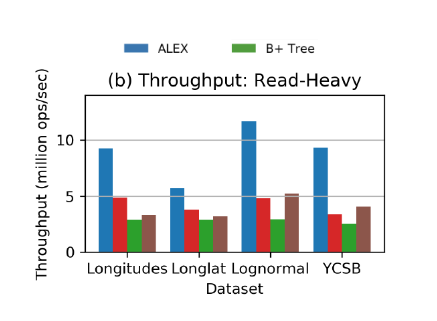
\includegraphics[width=\linewidth]{Figures/readheavy.png}
        \caption{Paper's results}
        \label{fig:readheavy_paper}
    \end{subfigure}
    \begin{subfigure}{0.3\textwidth}
        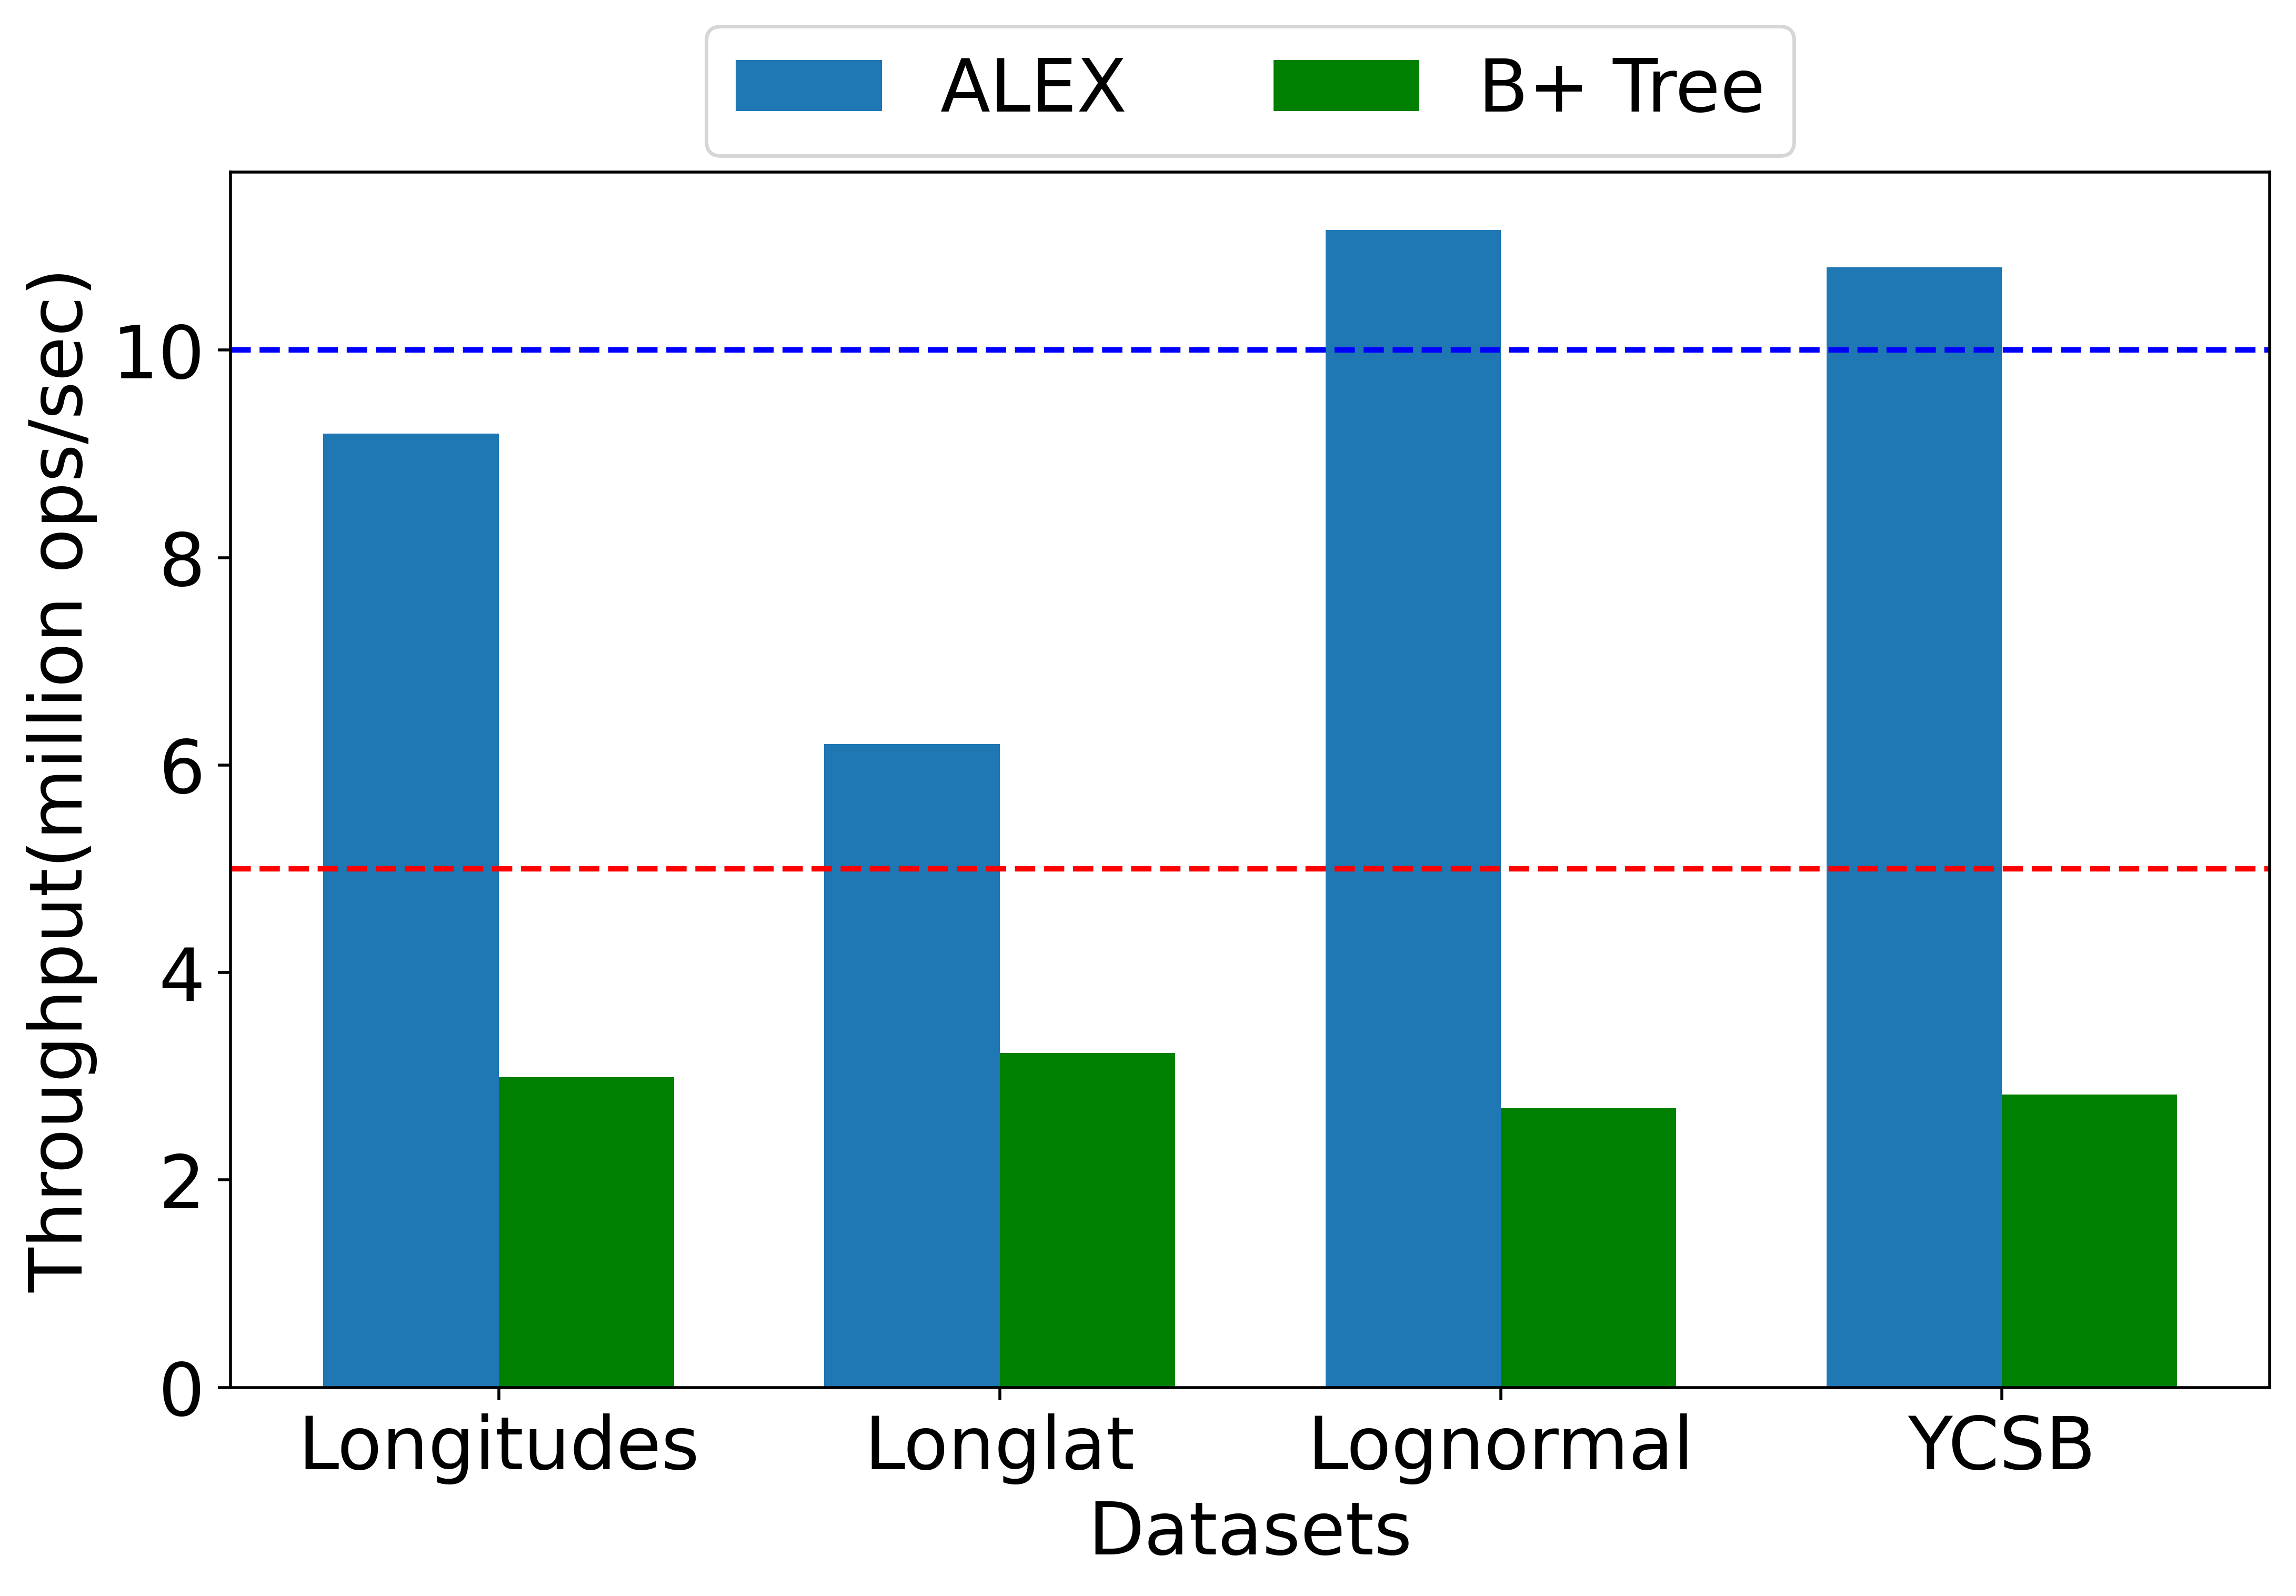
\includegraphics[width=\linewidth]{Figures/Readheavy (3).png}
        \caption{Our result}
        \label{fig:readheavy_our}
    \end{subfigure}
    \begin{subfigure}{0.35\textwidth}
        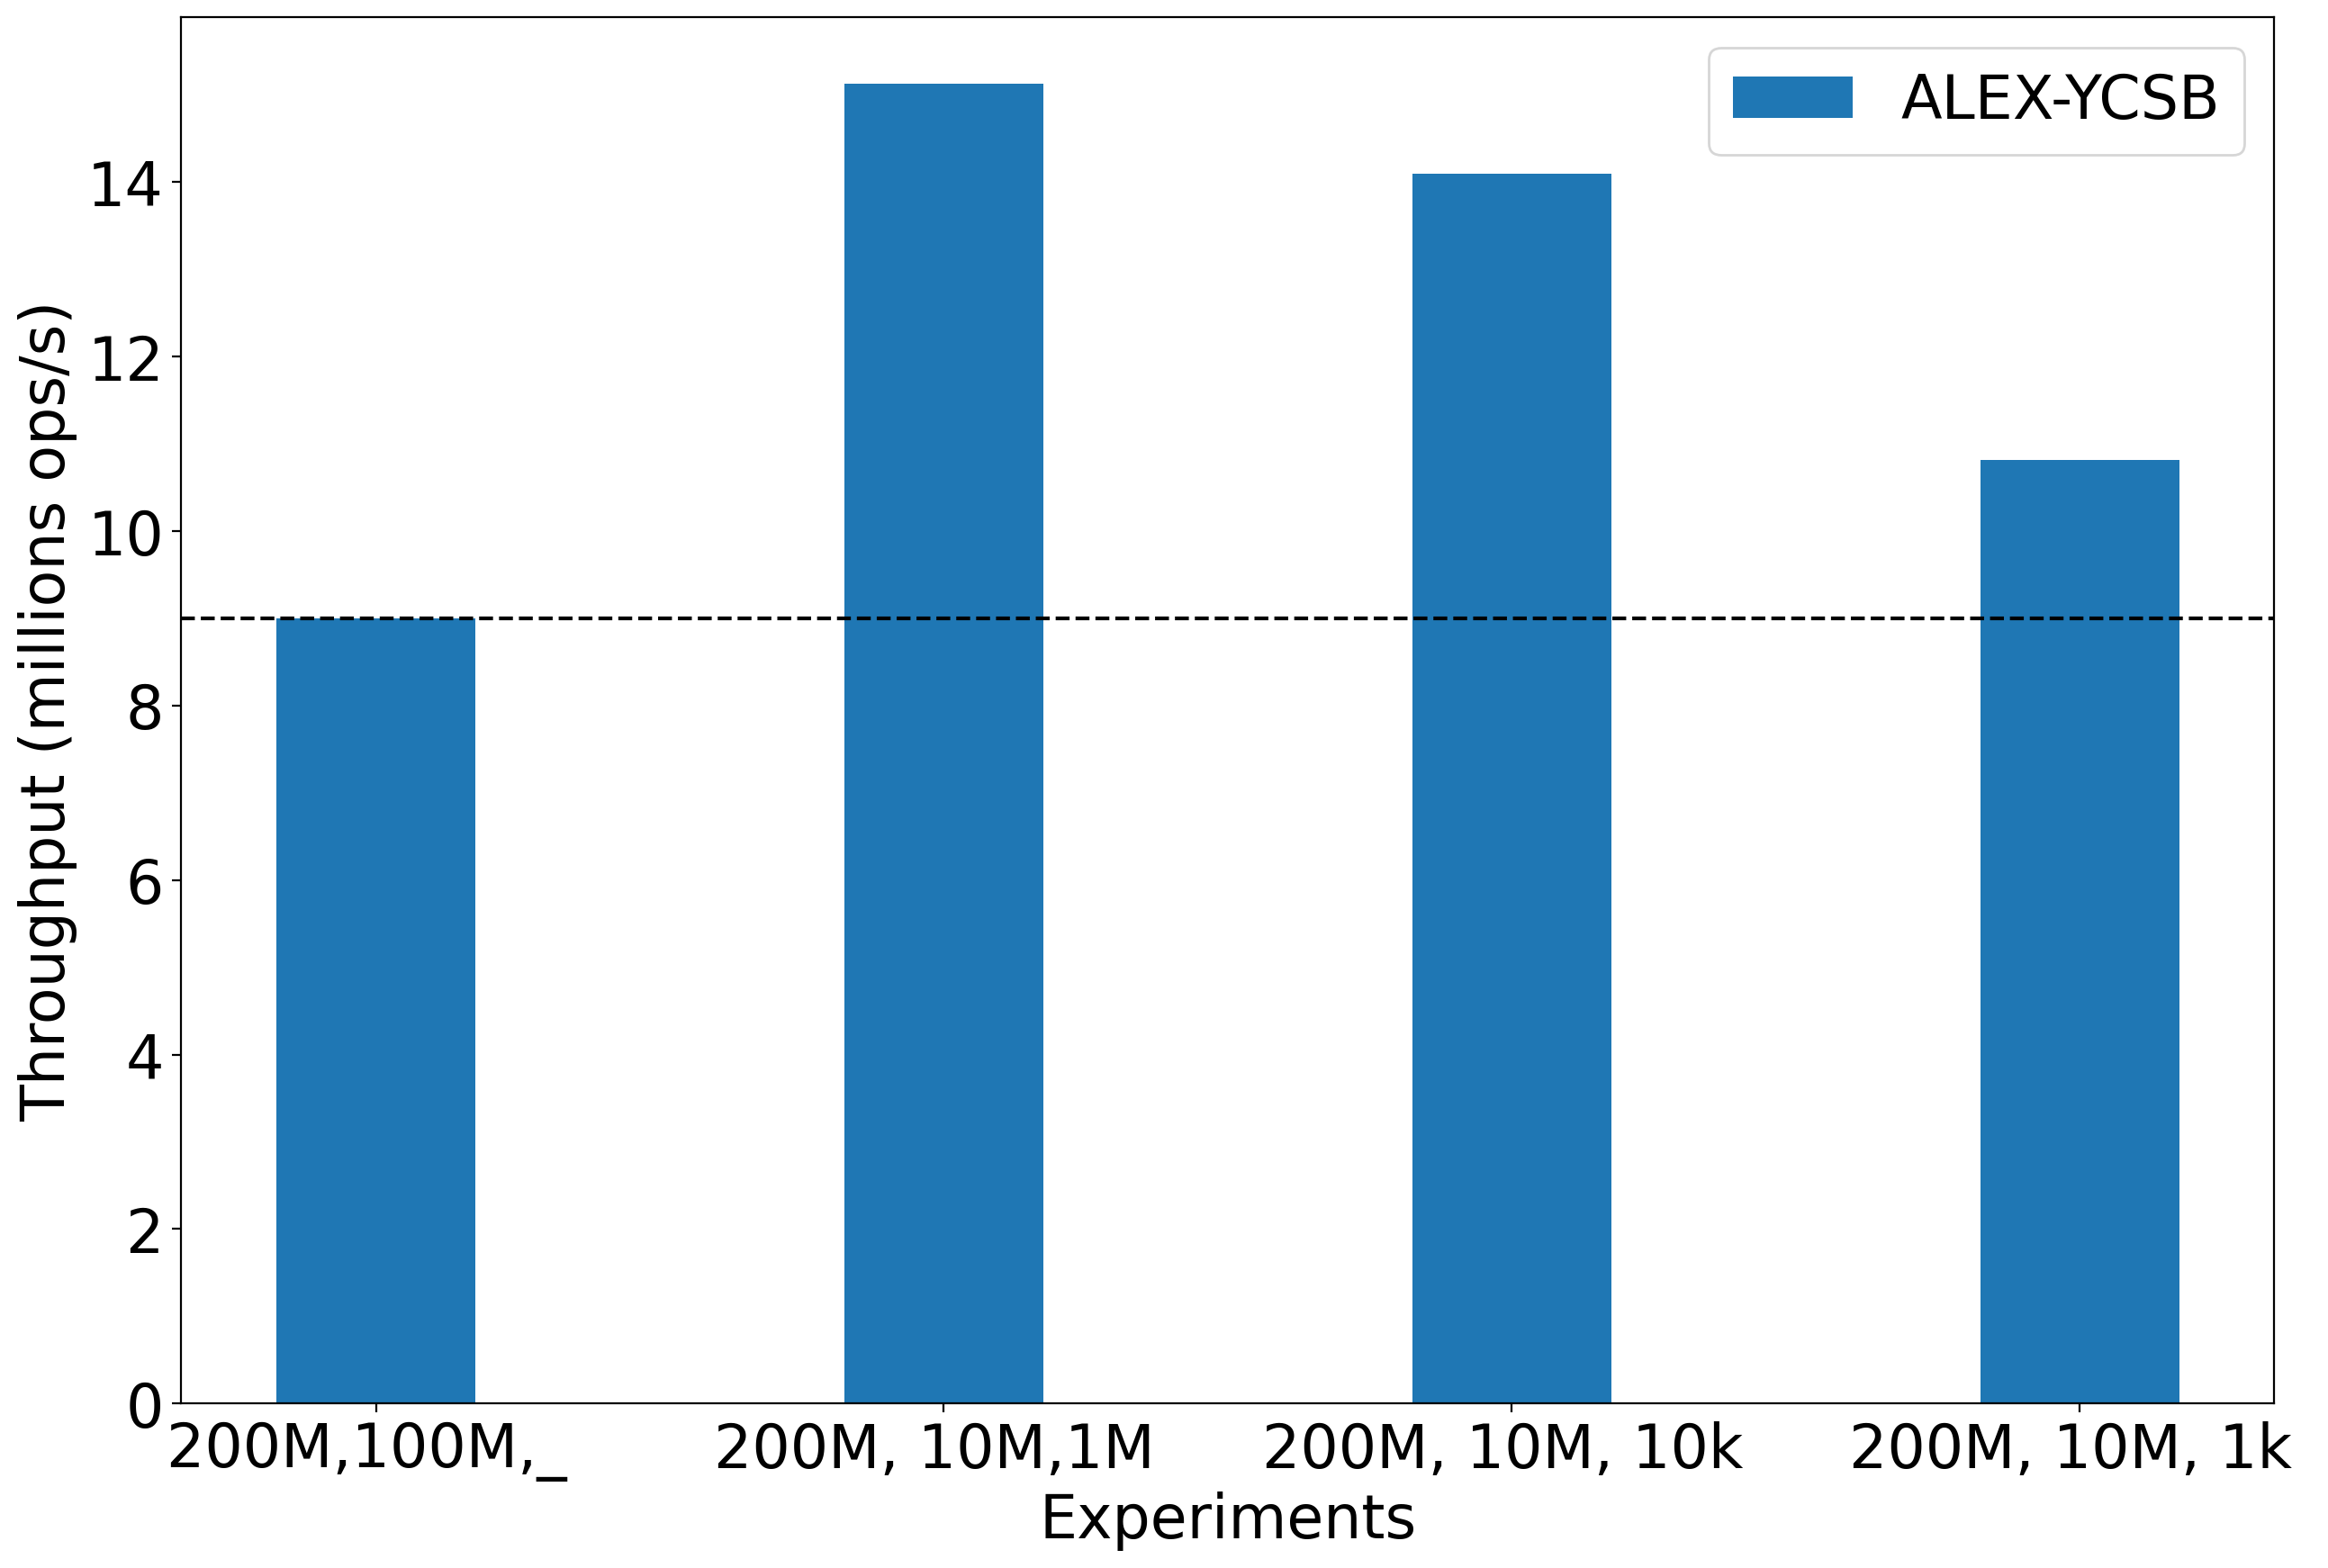
\includegraphics[width=\linewidth]{Figures/téléchargement.png}
        \caption{Batch size variation for YCSB}
        \label{fig:batchsize_variation}
    \end{subfigure}

    \caption{Read-Heavy workload experiments.}
    \label{fig:readheavy_experiments}
\end{figure}


\begin{figure}[htbp]
    

    \begin{subfigure}{0.3\textwidth}
        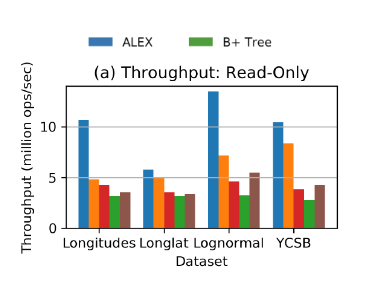
\includegraphics[width=\linewidth]{Figures/readonlu.png}
        \label{paper's result readonly}
        \caption{Paper's result}
    \end{subfigure}
    \begin{subfigure}{0.3\textwidth}
        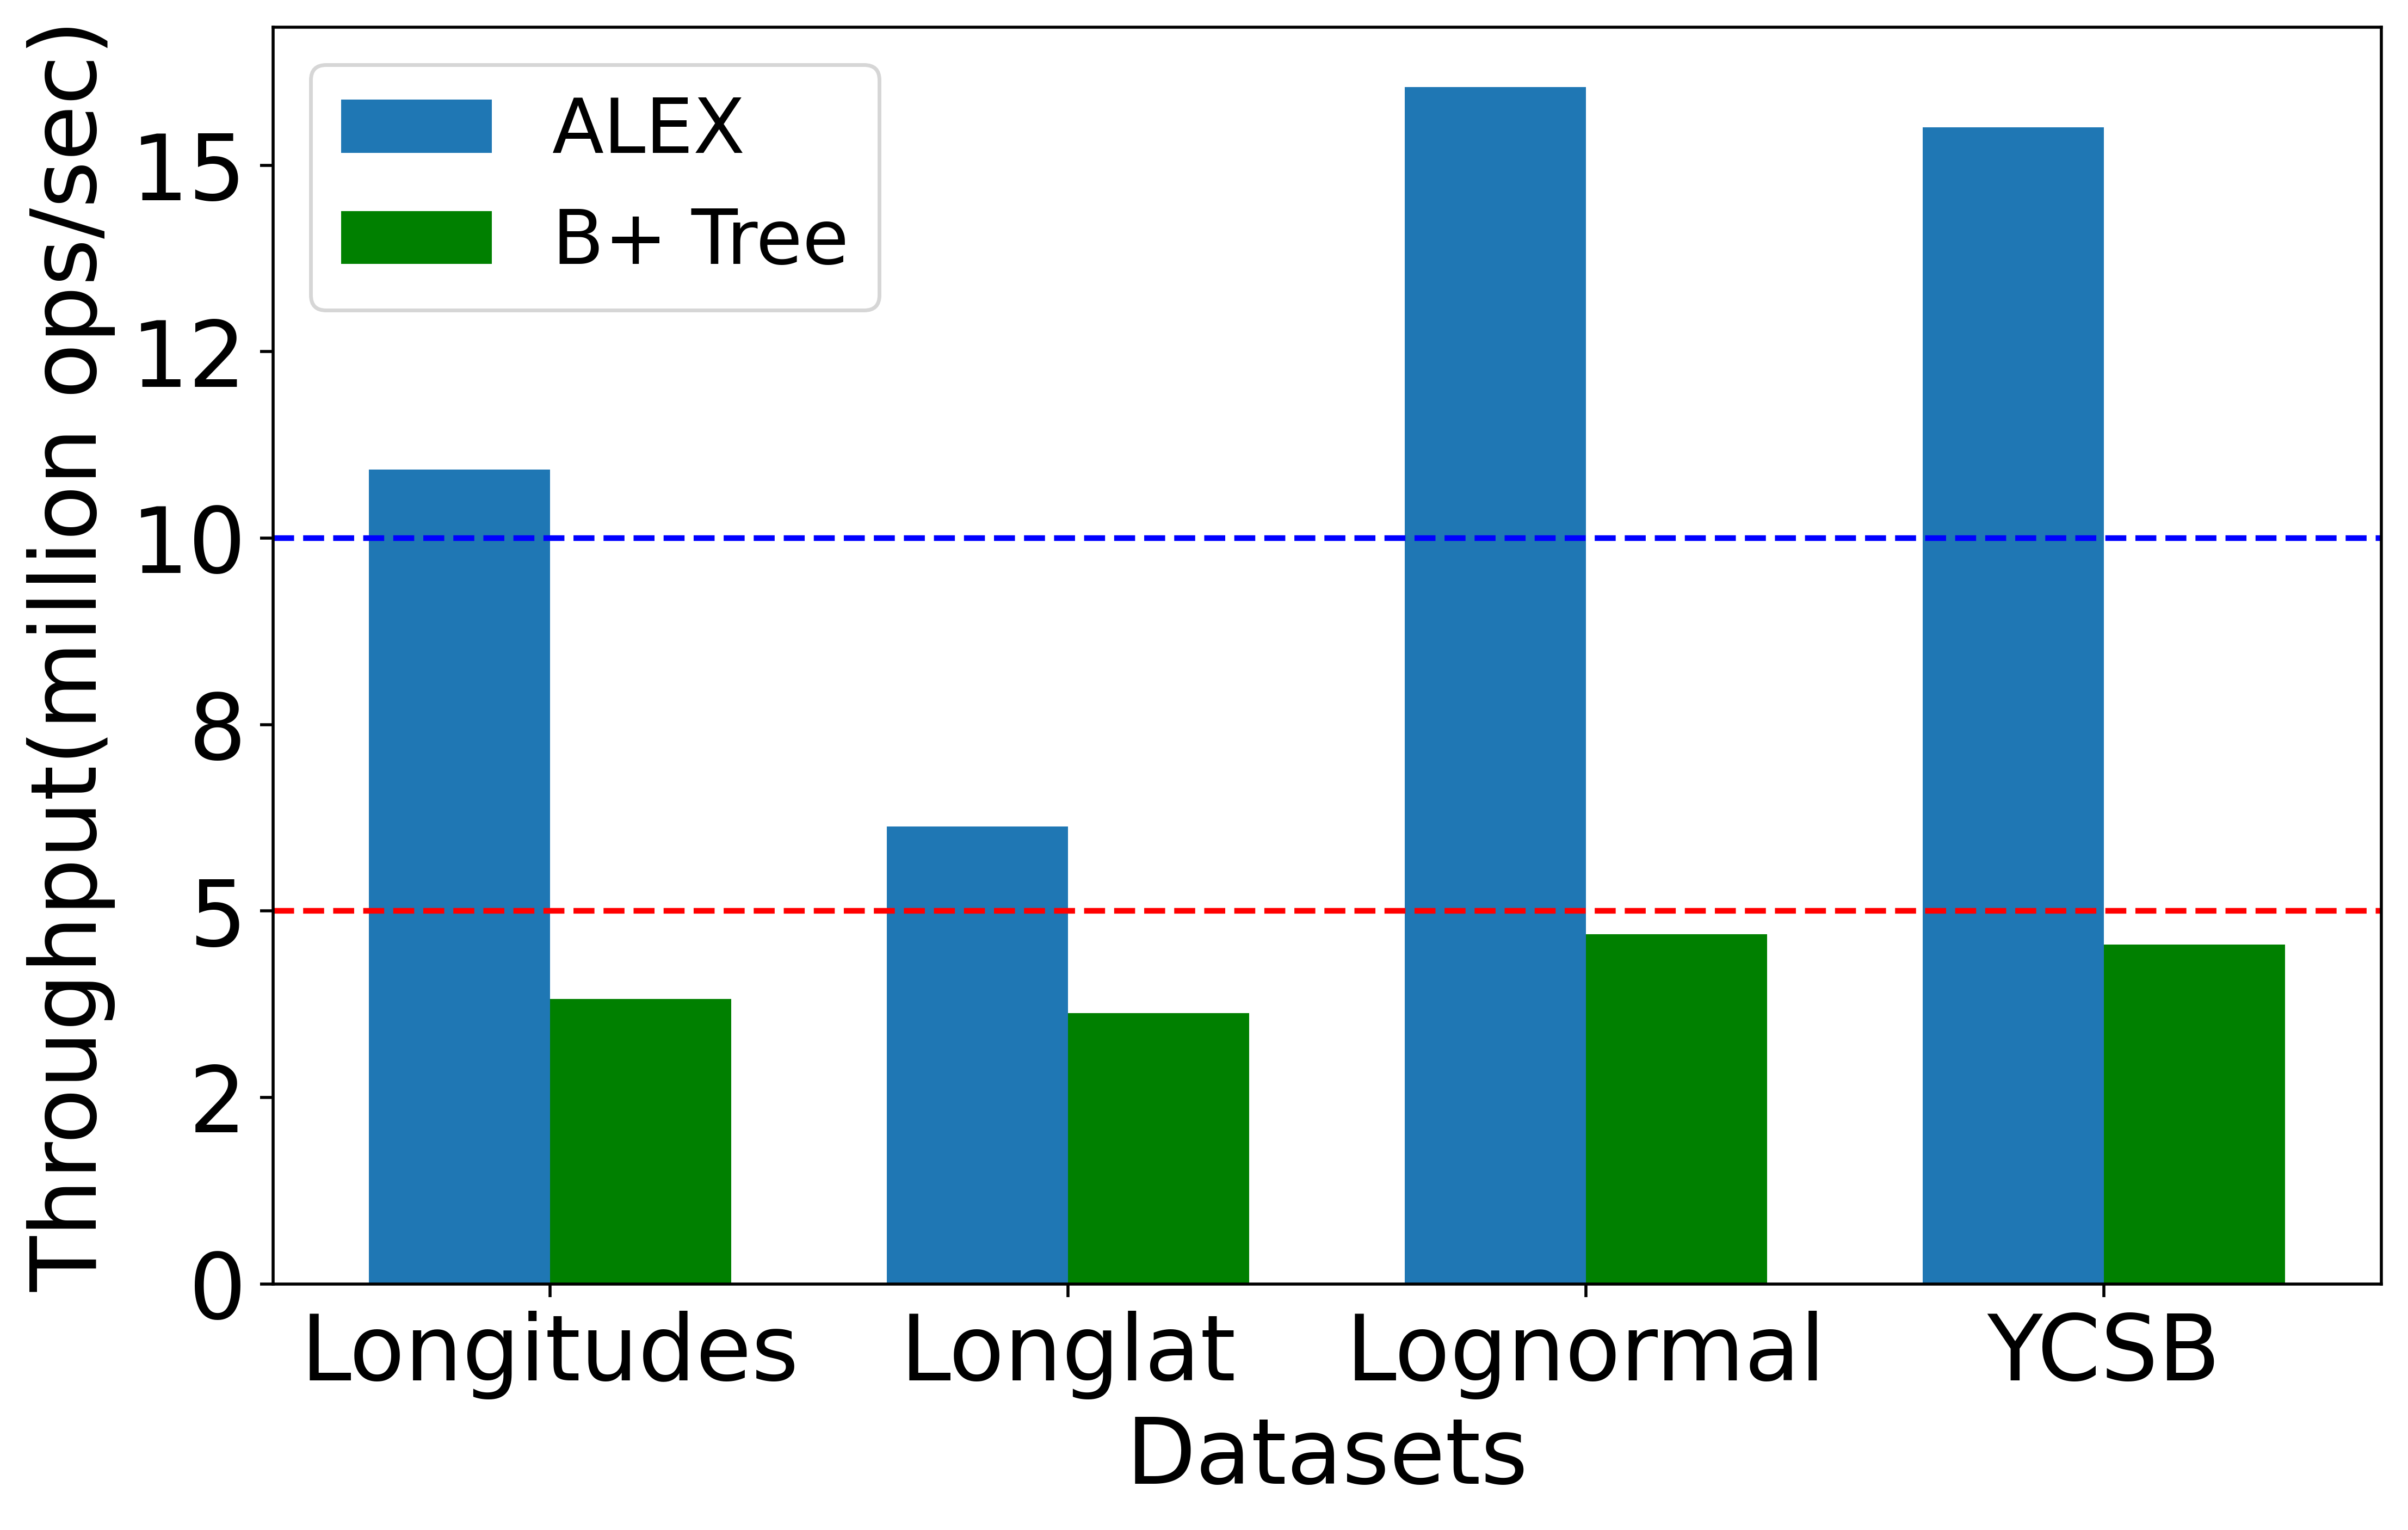
\includegraphics[width=\linewidth]{Figures/Readonly.png }
        \label{our result readonly}
        \caption{Our result}
        
    \end{subfigure}
    \begin{subfigure}{0.35\textwidth}
        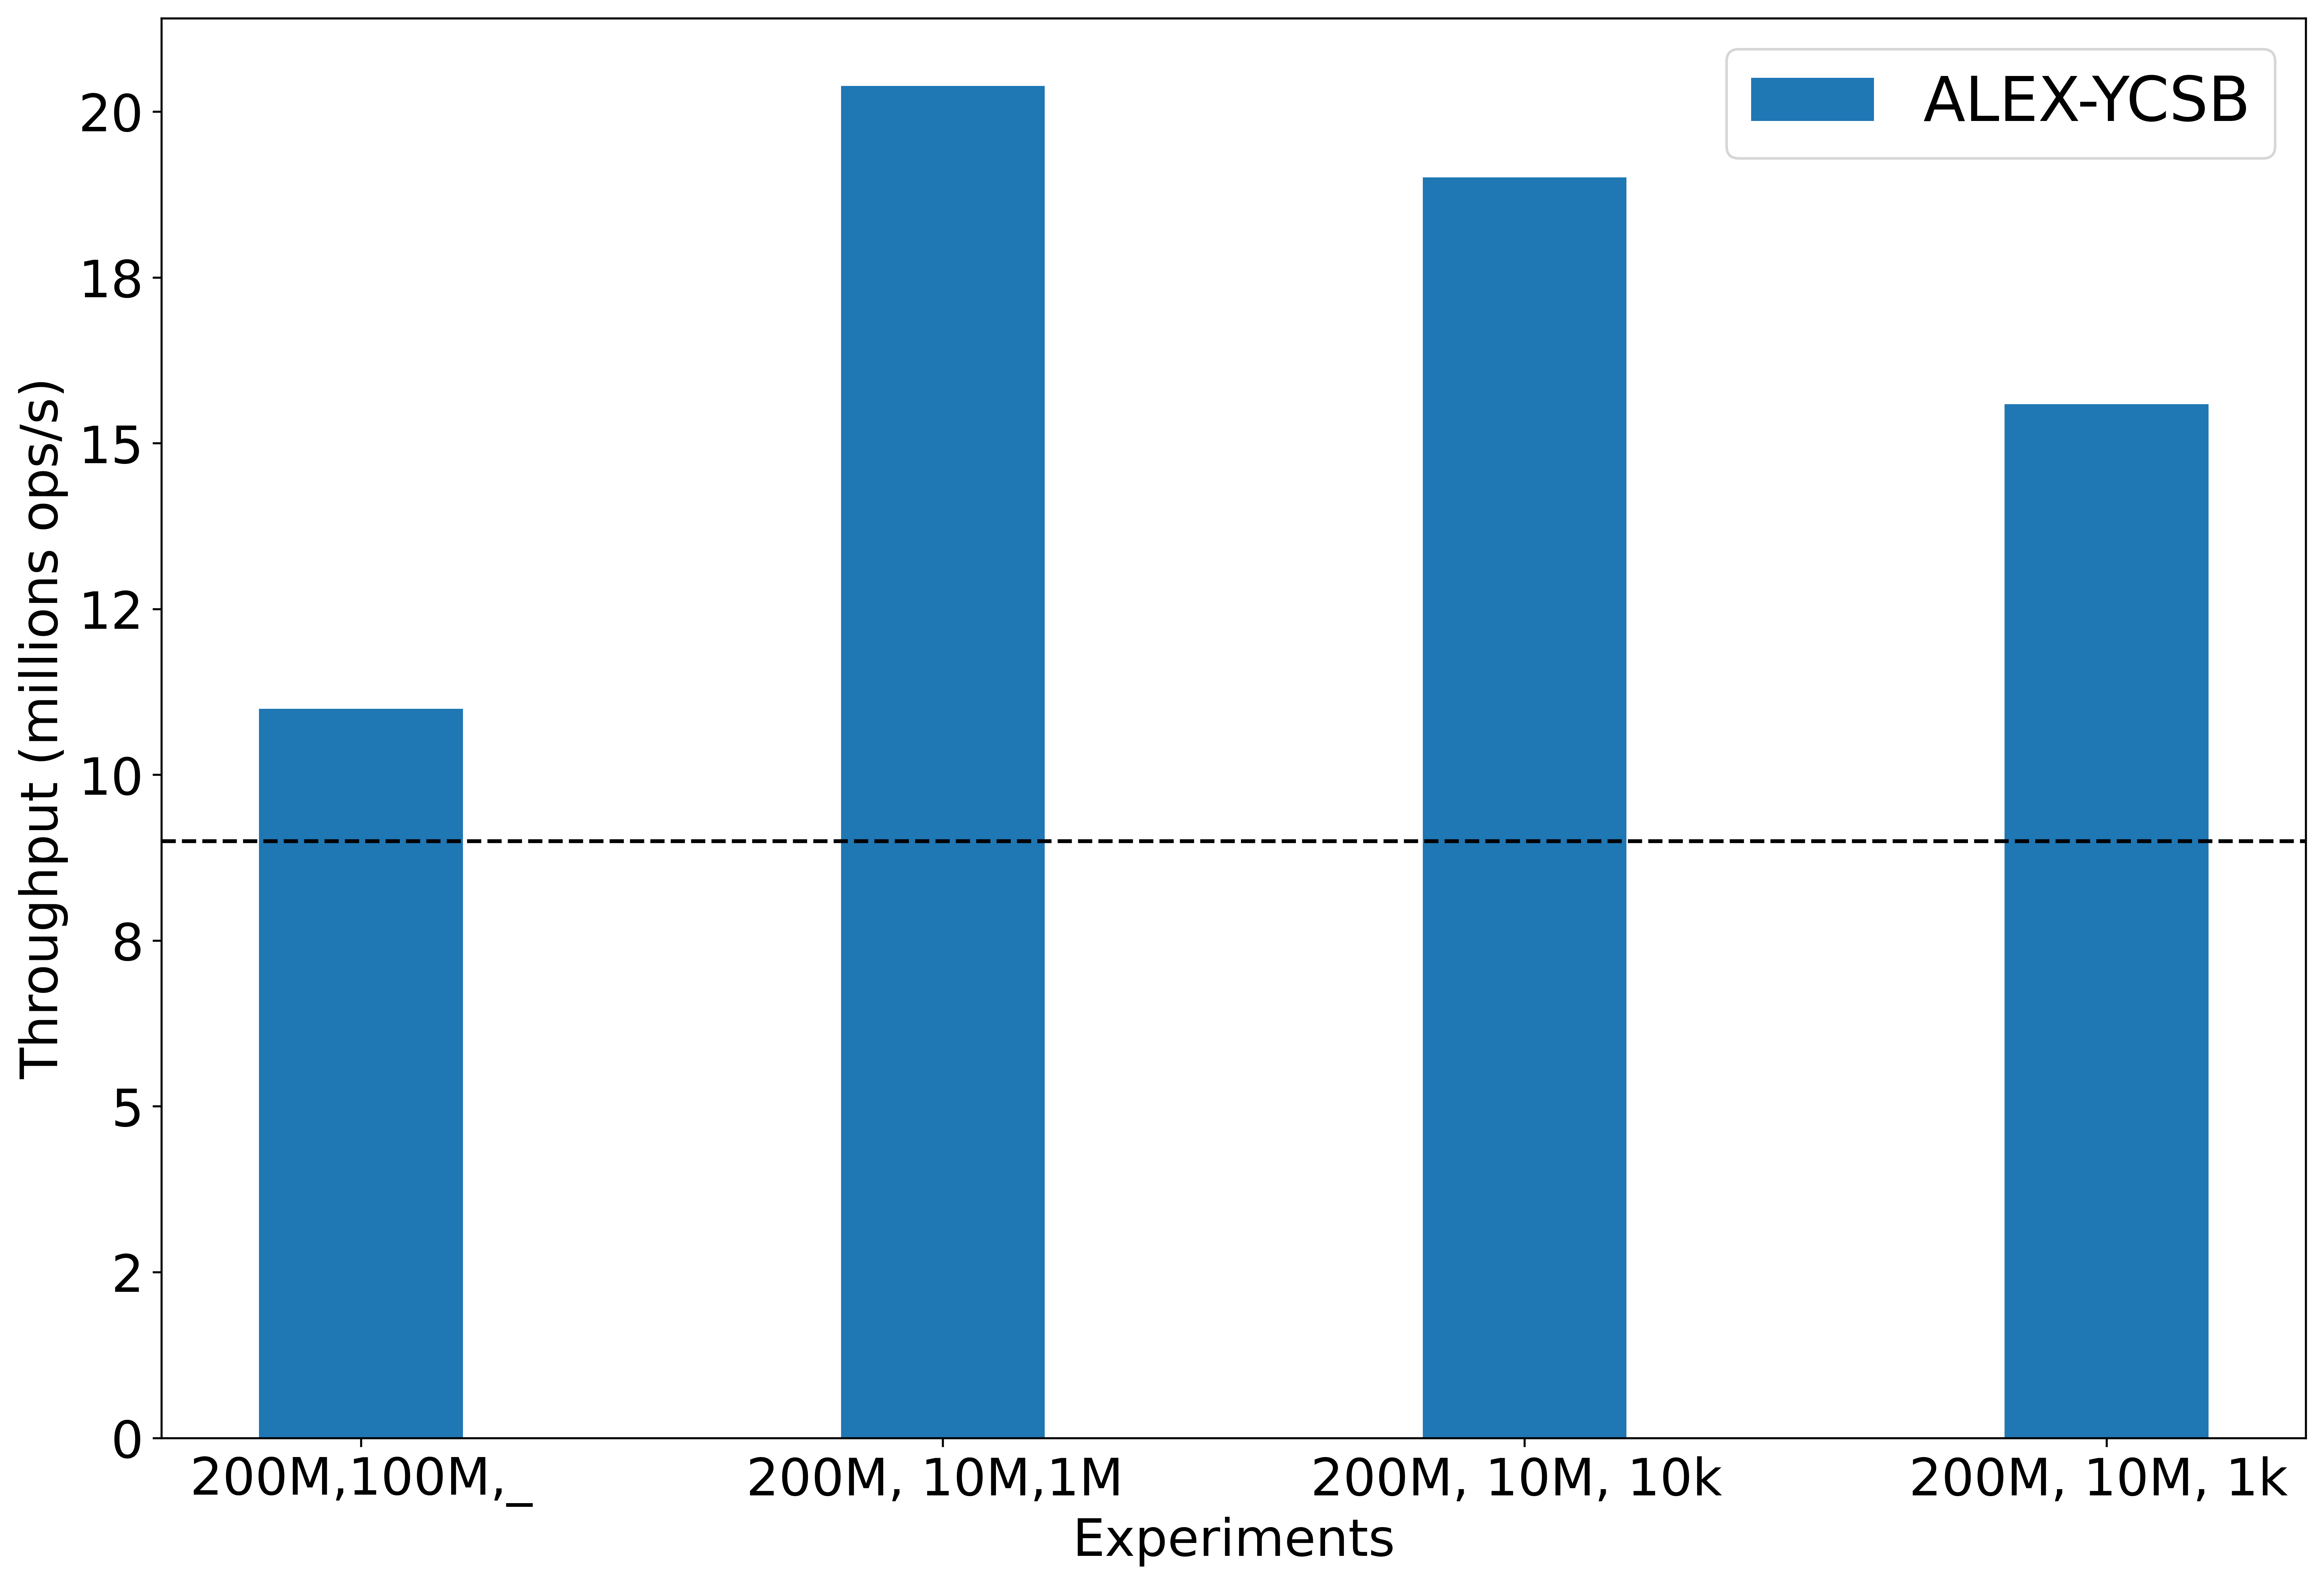
\includegraphics[width=\linewidth]{Figures/Batchsize_readonly.png}
        \caption{Batch size variation for YCSB  }
        \label{batch size read only}
    \end{subfigure}

    \caption{Read-Only workload experiments.}
    \label{fig:readonly_experiments}
\end{figure}


\begin{figure}[htbp]
    \centering

    \begin{subfigure}{0.3\textwidth}
        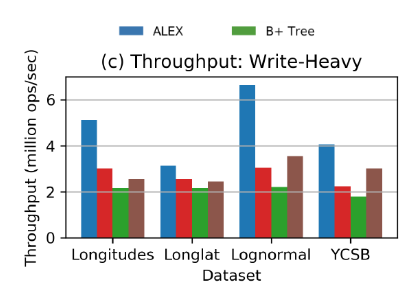
\includegraphics[width=\linewidth]{Figures/write heavy.png}
        \caption{Paper's result}
        \label{paper's result write heavy}
    \end{subfigure}
    \begin{subfigure}{0.3\textwidth}
        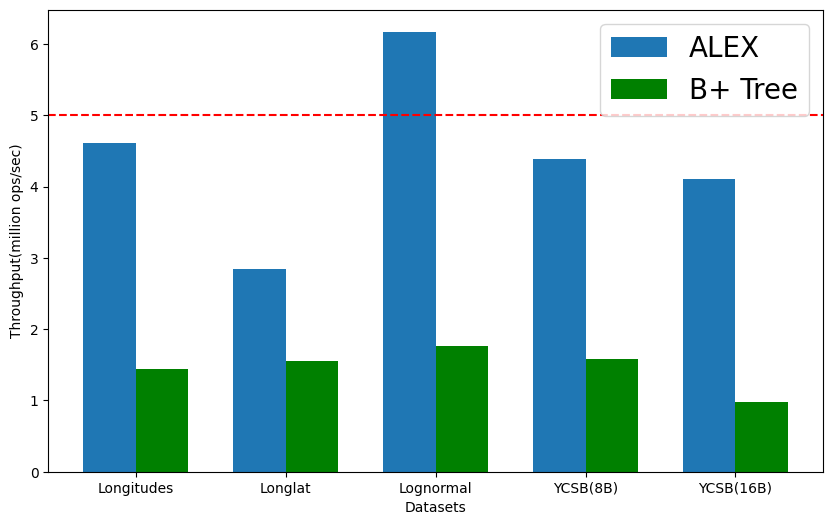
\includegraphics[width=\linewidth]{Figures/Writeheavy.png }
        \caption{Our result with varying payload size (8B to 16B) for YCSB}
        \label{Our result with varying payload size (8B to 16B) for YCSB}
    \end{subfigure}
  

    \caption{Write heavy workload experiments.}
\end{figure}


\begin{figure}[htbp]
    \centering

    \begin{subfigure}{0.3\textwidth}
        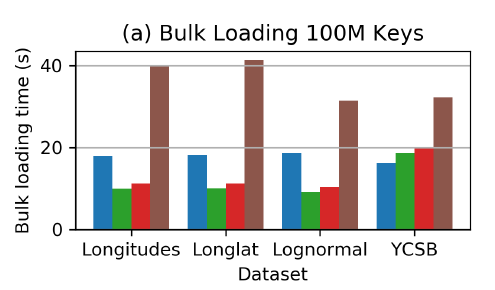
\includegraphics[width=\linewidth]{Figures/bulk loading time.png}
        \caption{Paper's result}
    \end{subfigure}
    \begin{subfigure}{0.3\textwidth}
        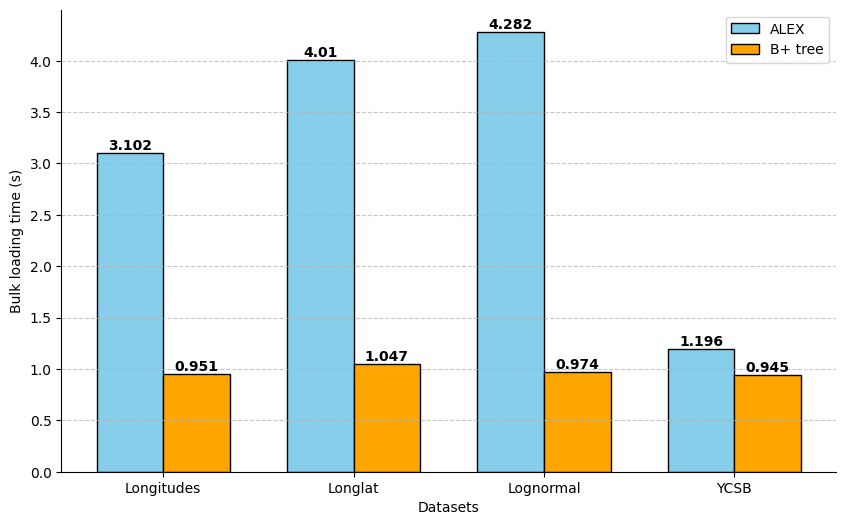
\includegraphics[width=\linewidth]{Figures/Bulkloadingtime (1).png }
        \caption{Our result (with 10M keys)}
    \end{subfigure}
  

    \caption{Bulk loading time experiments.}
\end{figure}


\subsection{Parameters of the experiments}
\begin{itemize}
    \item \textit{Longlat:} 200M total keys, 10M \textit{init\_num\_keys}, 1M batch size
    \item \textit{Longitudes:} 200M total keys, 10M \textit{init\_num\_keys}, 1M batch size
    \item \textit{Lognormal:} 190M total keys, 10M \textit{init\_num\_keys}, 1M batch size
    \item \textit{Ycsb:} 200M total keys, 10M \textit{init\_num\_keys}, 1k batch size
\end{itemize}

\subsection{Read-only workloads}
In Figure \ref{fig:readonly_experiments}, we managed to reproduce the results closely for Longitudes, Longlat and Lognormal datasets. For Ycsb, the throughput obtained was higher than the one in the paper. We ran the experiment and recorded the cumulative readings after one minute because there was no stopping criteria based on the number of insertions per batch in our benchmarking script. This experiment would not scale on the same setup we used in the following instances: i) if the size of payload was larger, ii) if the number of keys was 100x, iii) if the size of keys was larger, iv) if the data type was different (suppose, we were indexing images instead). This is because we worked with limited memory of 16GB which cannot accommodate aforementioned components.

\subsection{Read-heavy workloads}
In Figure \ref{fig:readheavy_experiments}, except for Ycsb, we were able to reproduce the results closely for other datasets under read-heavy workload (95\% reads and 5\% inserts) for both ALEX and B+ tree. We had initialized the index with 10M keys instead of 100M keys (both for ALEX and B+ tree). Interestingly, we observed similar throughput as the paper. Having less keys \emph{init\_num\_keys} in the index should have negatively impacted the throughput of the read-heavy workloads because our experiments should have experienced more misses in the cache. With greater \emph{init\_num\_keys}, we would have obtained a wider B+ tree with less depth, possibly making the search in the tree faster. We believe this is because the benchmarking script records the operations for throughput even if the keys are not found during reads (since the read values are not validated at any point). Had the number of keys in the workload been 100x and assuming bulk loading still worked, we would definitely see a difference in the performance because our 16GB memory would be insufficient. The throughput would exponentially go down because operations would have been held up due to page swaps.

\subsection{Write-heavy workloads}
Except the for Ycsb workload (explained separately in the following section), we observed that all the workloads showed slightly less throughput in comparison to the paper. This is especially true for B+ tree. It is to be noted that in the paper, the authors determined the most optimal page size for B+ tree to give the best performance on their setup. Instead, we proceeded with the default values without tuning the page size using grid search. Building on the reasoning from the previous subsection, the indexes constructed by authors (both B+ tree and ALEX) were having lesser depth because they used a higher number of \emph{init\_num\_keys} during the bulk loading phase. In our experiments, the indexes created would have been less wide and more deep leading to greater search time. This means the inserts would take some penalty and as such write-heavy workloads are expected to display slightly lesser throughput compared to the experiments in the paper.


\subsection{Bulk loading time}
We calculated the bulk loading time as follows: Adding the time it takes to sort the keys and the time taken by the bulk loading function of B+ tree/ ALEX. Since we loaded only 10M keys instead of 100M keys, we expected to take less time in our experiments for bulk loading the data in the indexes. We expected to our experiments to be faster in bulk loading by a factor of 10. We found that it was largely true for ALEX. We observed some deviation for Ycsb workload. It was slightly faster than the bulk loading time in the paper. We believe this was because the size of payload being generated randomly in our experiments was limited to 8 bytes so it was quicker to bulk load smaller payloads in comparison to 80 bytes done in the actual experiment. For B+ tree, both the observations in terms of bulk loading times being smaller by a factor of 10 and Ycsb exhibiting a quicker performance also hold true.

\subsection{Deviations for Ycsb}
We used 8 bytes payload for Ycsb as opposed to 80 bytes payload used in the experiments. Further, we used 1k batch size for Ycsb. Our hypothesis was that since the payload we used was smaller than the one used in the paper, we should observe better performance for Ycsb in our experiments across all the workloads than the actual experiments. We found that if we use the parameters closely resembling the parameters used in the experiments, the observed throughput tends to be lesser and much closer to the performance seen in the paper. We also found that the throughput decreases for read heavy workloads over 10M init keys as we decrease the batch size for ycsb dataset. We did not use 80 bytes payload size because the memory in our machines would not have been sufficient to handle the workloads. We tried some experiments with a payload size of 16 bytes to test our hypothesis of greater the payload size, lesser the performance.

\subsection{Payload size variations}
It was the Ycsb dataset for which we saw most of the deviations across different workloads. Our hypothesis is that since we used a smaller payload (8 bytes) instead of 80 bytes used in the paper, we observed better performance. We further extrapolated that reducing the batch size leads to throughput decrease as described in the previous subsection. Due to memory limitations in our test setup, we could not replicate 80 bytes payload but we tried out the write-heavy workload with 16 bytes payload to gauge the effect on throughput of increased payload size. We found that using 16 bytes payload did indeed reduce the performance for ycsb write-heavy workloads for ALEX and B+ tree. We used a long double data type for payload and confirmed that it is indeed 16 bytes on our machine (teach-node-07) before proceeding with the measurements. Further, we also confirmed that increased payload size can lead to more time taken for bulk loading. We found that instead of 0.945 seconds for bulk loading (and sorting) 8 bytes payload, bulk loading (and sorting) took 1.303 seconds for 16 bytes payload for the same number of records (10M \emph{init\_num\_keys}).

\section{Discussion on Non-reproduced experiments}
Apart from the three workloads we reproduced for ALEX and B+ tree, we expect the write-only workload to also be reproducible in our environment because it just involves changing the number of inserts per batch to 100\% in our bench marking scripts. Also, it is to be noted that in read-only, read-heavy and write-heavy workloads, the reads consisted of a lookup of a single key. Further, we expect short range lookups to also be reproducible in our environment because the additional step involved after a key lookup is a scan of random selection of keys up to a max scan length of 100. The resource requirements for this workload are quite similar to the workloads we ran so far (per scan size - 100*key size of 8 bytes). We believe that since the dataset sizes were around \~1.5GB (average approximation), payload being 8 bytes and the throughput observation happening within 1 minute of running a workload; all the workloads can be run on our test setup. However, the bigger question is if the exact performance could be reproduced, the answer to which is a bit more nuanced.

We took the liberty of downsizing the \emph{init\_num\_keys} to 10M from 100M. We used 1M batch sizes for Longlat, Longitudes and Lognormal datasets instead of 1k. We used a smaller payload (8 bytes) for Ycsb instead of 80 bytes. All this helped us to make the bench marking quite feasible in our test setup but it is not scalable without increasing the resources currently present. Foremost, we would need more memory if we have to use parameters closer to what the paper has used. The index sizes for B+ tree can be calculated by counting the number of inner nodes (we counted the number of nodes) and tracking the node size. For ALEX, calculating the final index size (which we did not do) proved to be non-trivial as we would need to determine the sum of the sizes of all the models used, metadata and internal nodes. 

The experiments from figure-9 in the paper except index sizes are reproducible. Figure-10 from the paper should also be reproducible assuming we use the same config of payloads and datasets we used for experiments so far. Our memory can handle (per scan size - 1000*key size of 8 bytes). Figure-11 is not reproducible because bulk loading for 100M was not working on our setup. Similarly, figure-12 is also not reproducible because they are using 900M \emph{init\_num\_keys} in the experiment. Further, using 80 bytes payload for ycsb is not possible on our setup because (8 bytes key + 80 bytes payload) it would involve using 17.6GB memory which we do not possess.



\newpage
\bibliography{biblio} % Specify your .bib file name
\bibliographystyle{plainurl}
\end{document}